%!TEX root =  ../thesis.tex
% CHAPTER 1
\chapter{Introduction}
\label{chp:b1}

	There is an increasing interest in the early stages of design, the so called fuzzy front-end in design (FFED), which focuses on defining better questions before designers attempt to answer them \cite{aaltonenHowWeMake2005}.
	

	\begin{figure}[h!]
			\centering
			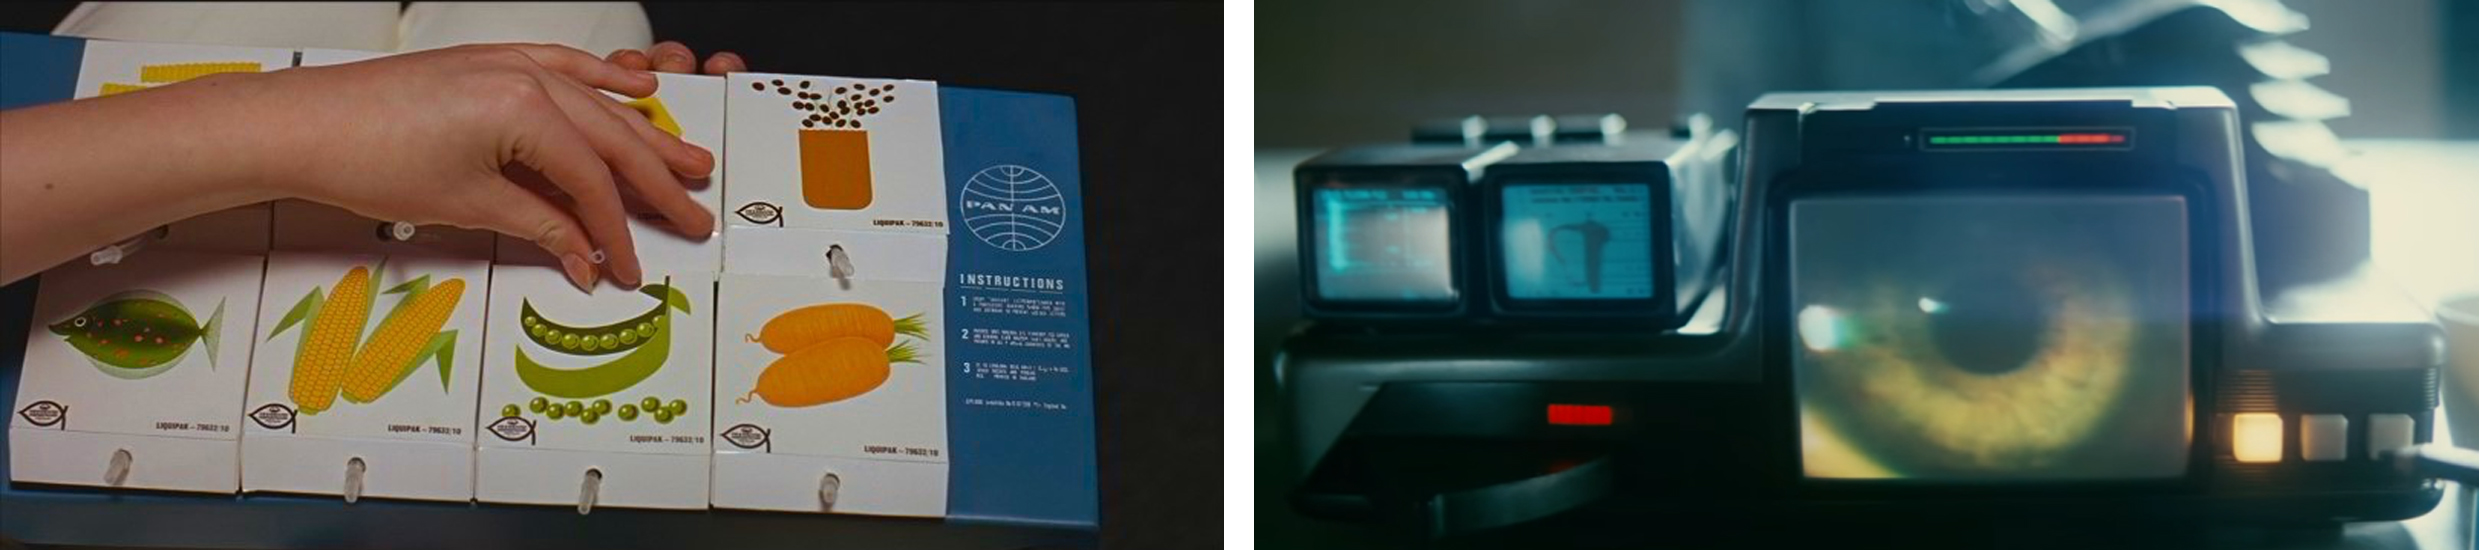
\includegraphics[width=.8\textwidth]{figures/2001-Bladerunner.jpg}
			\caption{Screencaps from a movie \cite{bladeRunner}.}
			\label{fig:movies}
	\end{figure}

	\begin{comment}
		TODO
		Buraya bir bağlantı lazım. Önceki paragrafta lafı design studentlara getirebilirsin.
	\end{comment}

	
	\section{Research Aim}
	

\section{Research Questions and Approach}
\label{Research Questions}
	My aim is to explore world building in design education, by understanding and supporting it in the early phases of design. My main research questions are as follows: 

	\begin{enumerate}
	\item How can a theoretical model describe and represent the world building process of design students when working with future contexts?
	\item What are the properties of a toolset for openly enabling world building to be used by design students when working with future contexts?
	\end{enumerate}


\section{Contributions to Literature}

	There will be two main contributions to the existing body of knowledge in design education. First, the answer to my first research question will provide a theoretical model of world building in design education. This model will be generated by layering four research outputs: (1) an interpretive literature review for transporting concepts of world building from media studies to design, (2) elements and their properties of world building, (3) processes of world building and (4) pragmatic concerns of world building. These layers will be weaved together to present a wholistic model of world building in design education, contributing to existing body of knowledge within design education literature.
	

\section{Structure of the Thesis}
	The overall structure of this dissertation is built on four components: literature review, methodological framework, workshops and conclusions. The literature review consists of Chapter~\ref{chp:b2} (p.~\pageref{chp:b2}), and Chapter~\ref{chp:b3} (p.~\pageref{chp:b3}). These chapters will present my theoretical background. 
